\section{Conclusion}

This article comes last in a series of three articles where we investigate for
a more biologically plausible self-organization. 





\section*{Abbreviations}
\begin{description}
    \item[\bf SOM] Self-organizing Map
    \item[\bf BMU] Best matching unit
    \item[\bf DSOM] Dynamic Self-organizing Map
\end{description}





%% \begin{figure}
%%   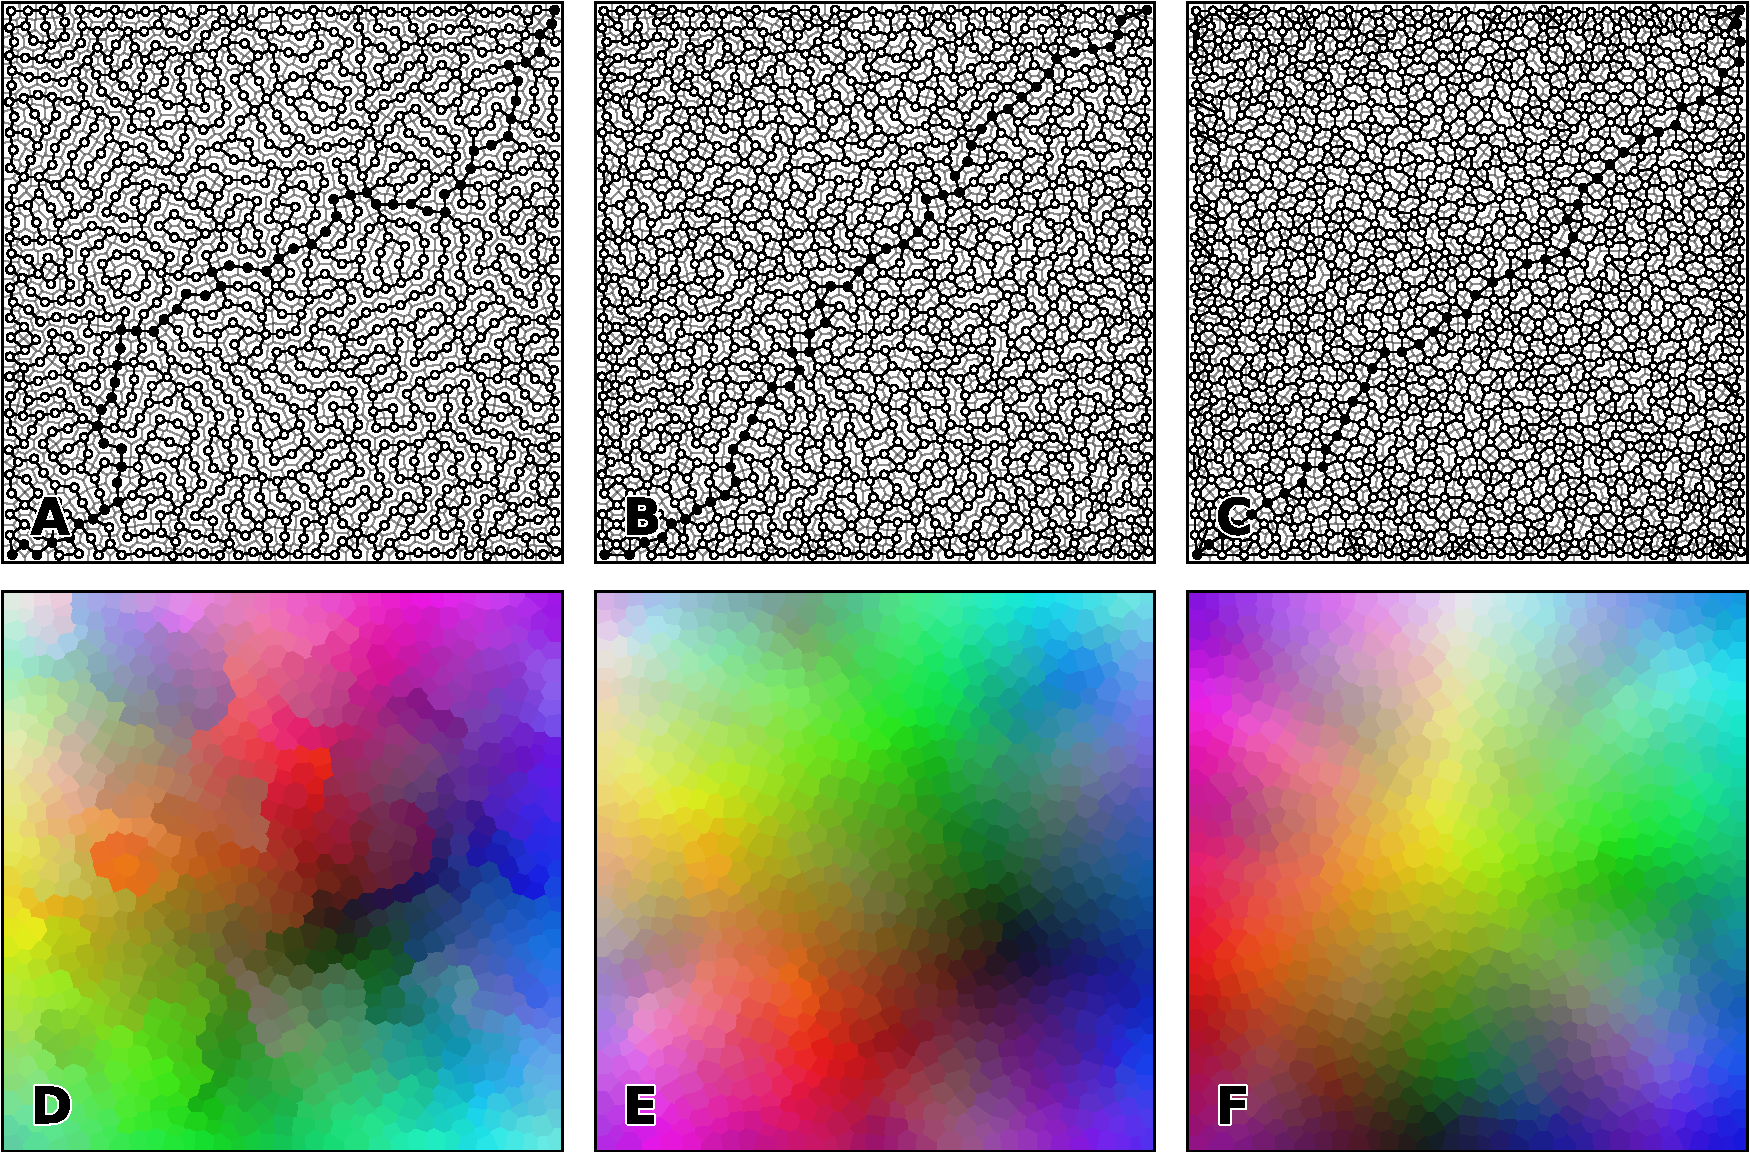
\includegraphics[width=\columnwidth]{figures/vsom-topology.pdf}

%%   \caption{\textbf{Influence of topology on the self organization.} The same
%%     initial set of 1003 neurons has been equiped with 2-nearest neighbors, 3
%%     nearest neighbors and 4-nearest neighbors induced topology (panels
%%     \textbf{A}, \textbf{B} and \textbf{C} respectively) and trained on 25,000
%%     random RGB colors. This lead to qualitatively different self-organization
%%     as shown on panels \textbf{D}, \textbf{E} and \textbf{F} respectively, with
%%     major discontinuities in the 2-nearest neighbors case. A sample path from
%%     the the lower-left neuron to the upper-right neuron has been highlighted with
%%     a thick line (with respective lengths of 59, 50 and 46 nodes).}
%% \end{figure}

%% \begin{figure}
%%   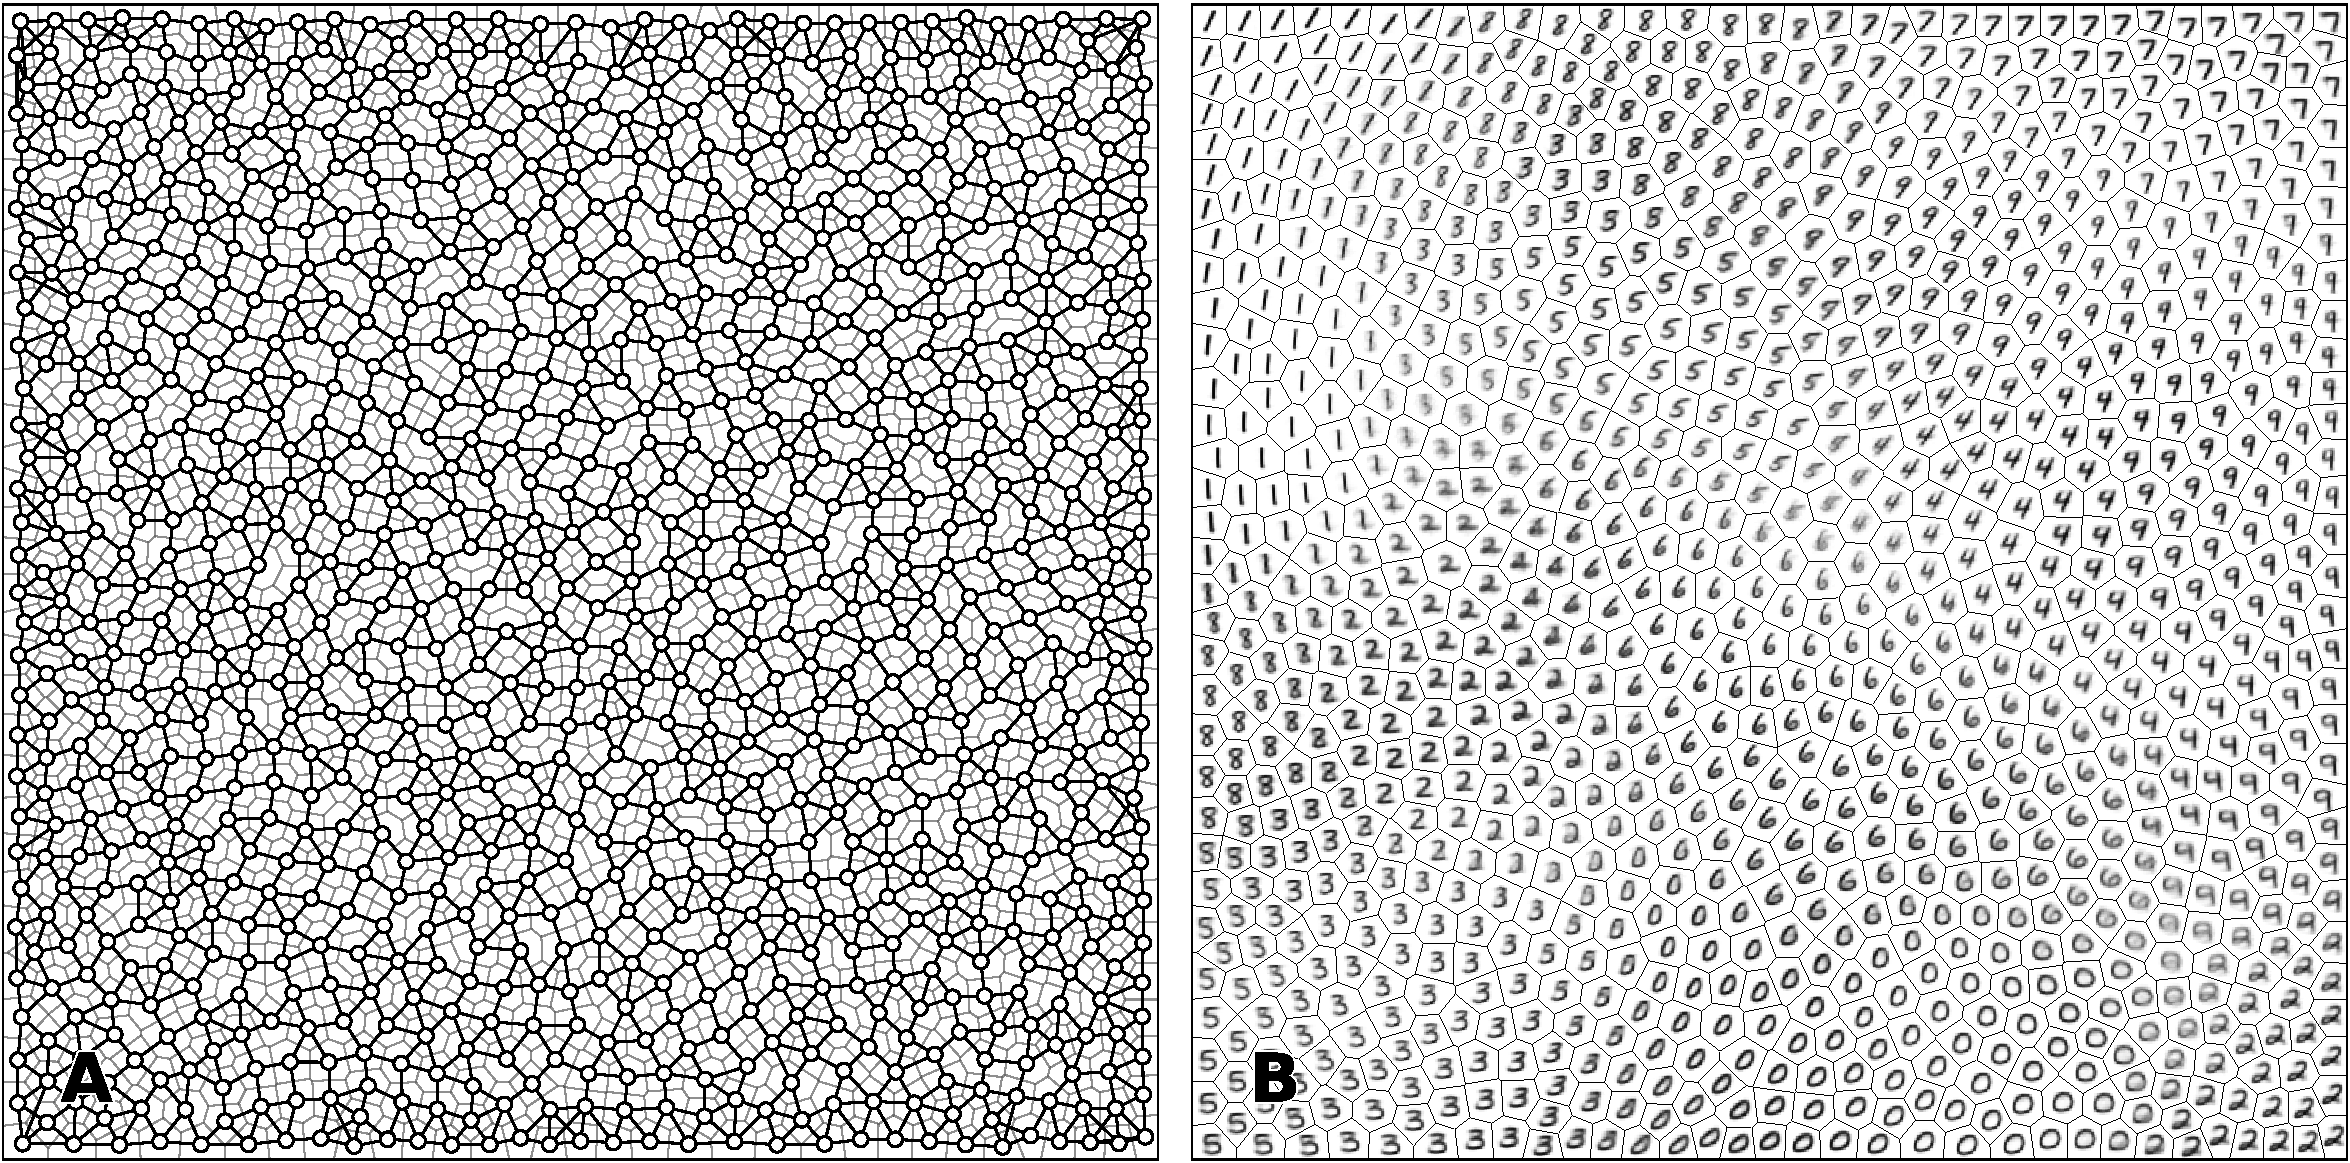
\includegraphics[width=\columnwidth]{figures/vsom-mnist-1.pdf}

%%   \vspace{2mm}
  
%%   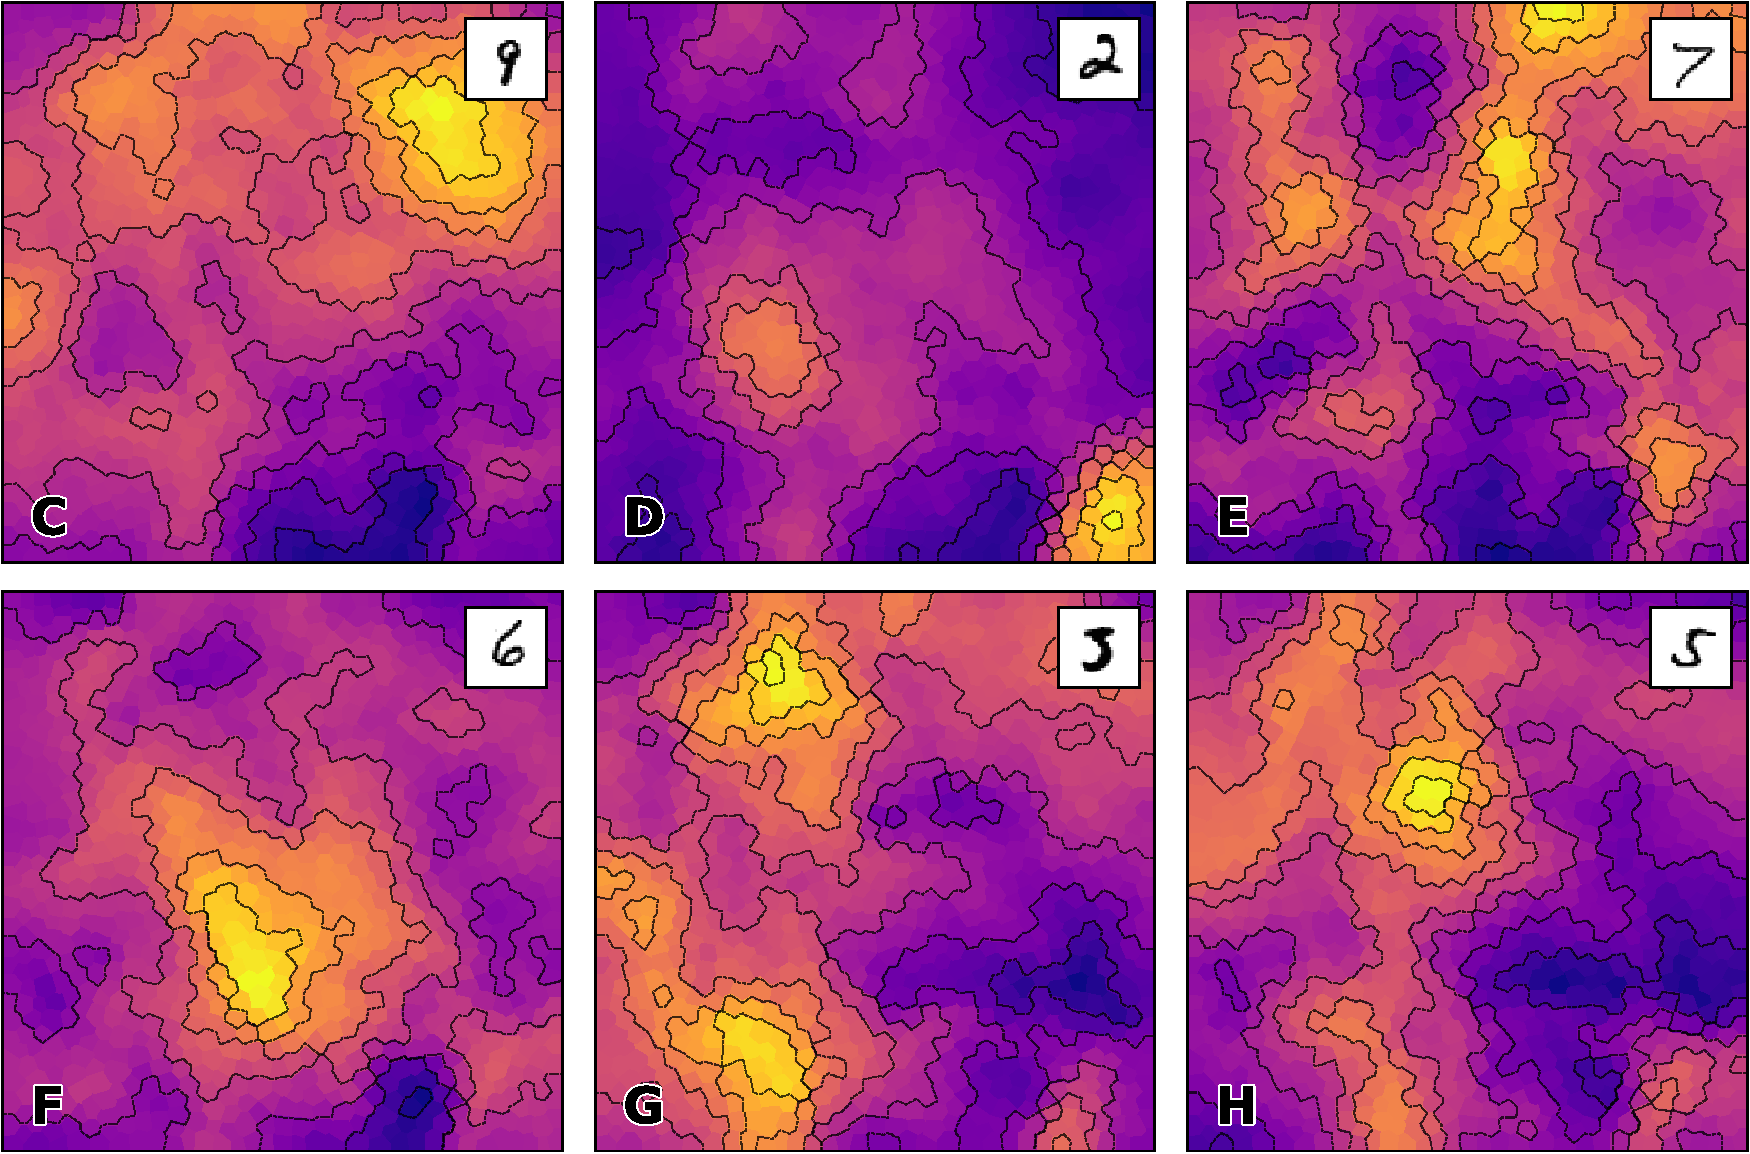
\includegraphics[width=\columnwidth]{figures/vsom-mnist-2.pdf}

%%   \vspace{2mm}

%%   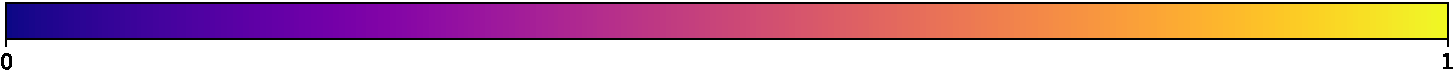
\includegraphics[width=\columnwidth]{figures/colormap.pdf}

%%   \caption{}
%% \end{figure}


%% \begin{figure}
%%   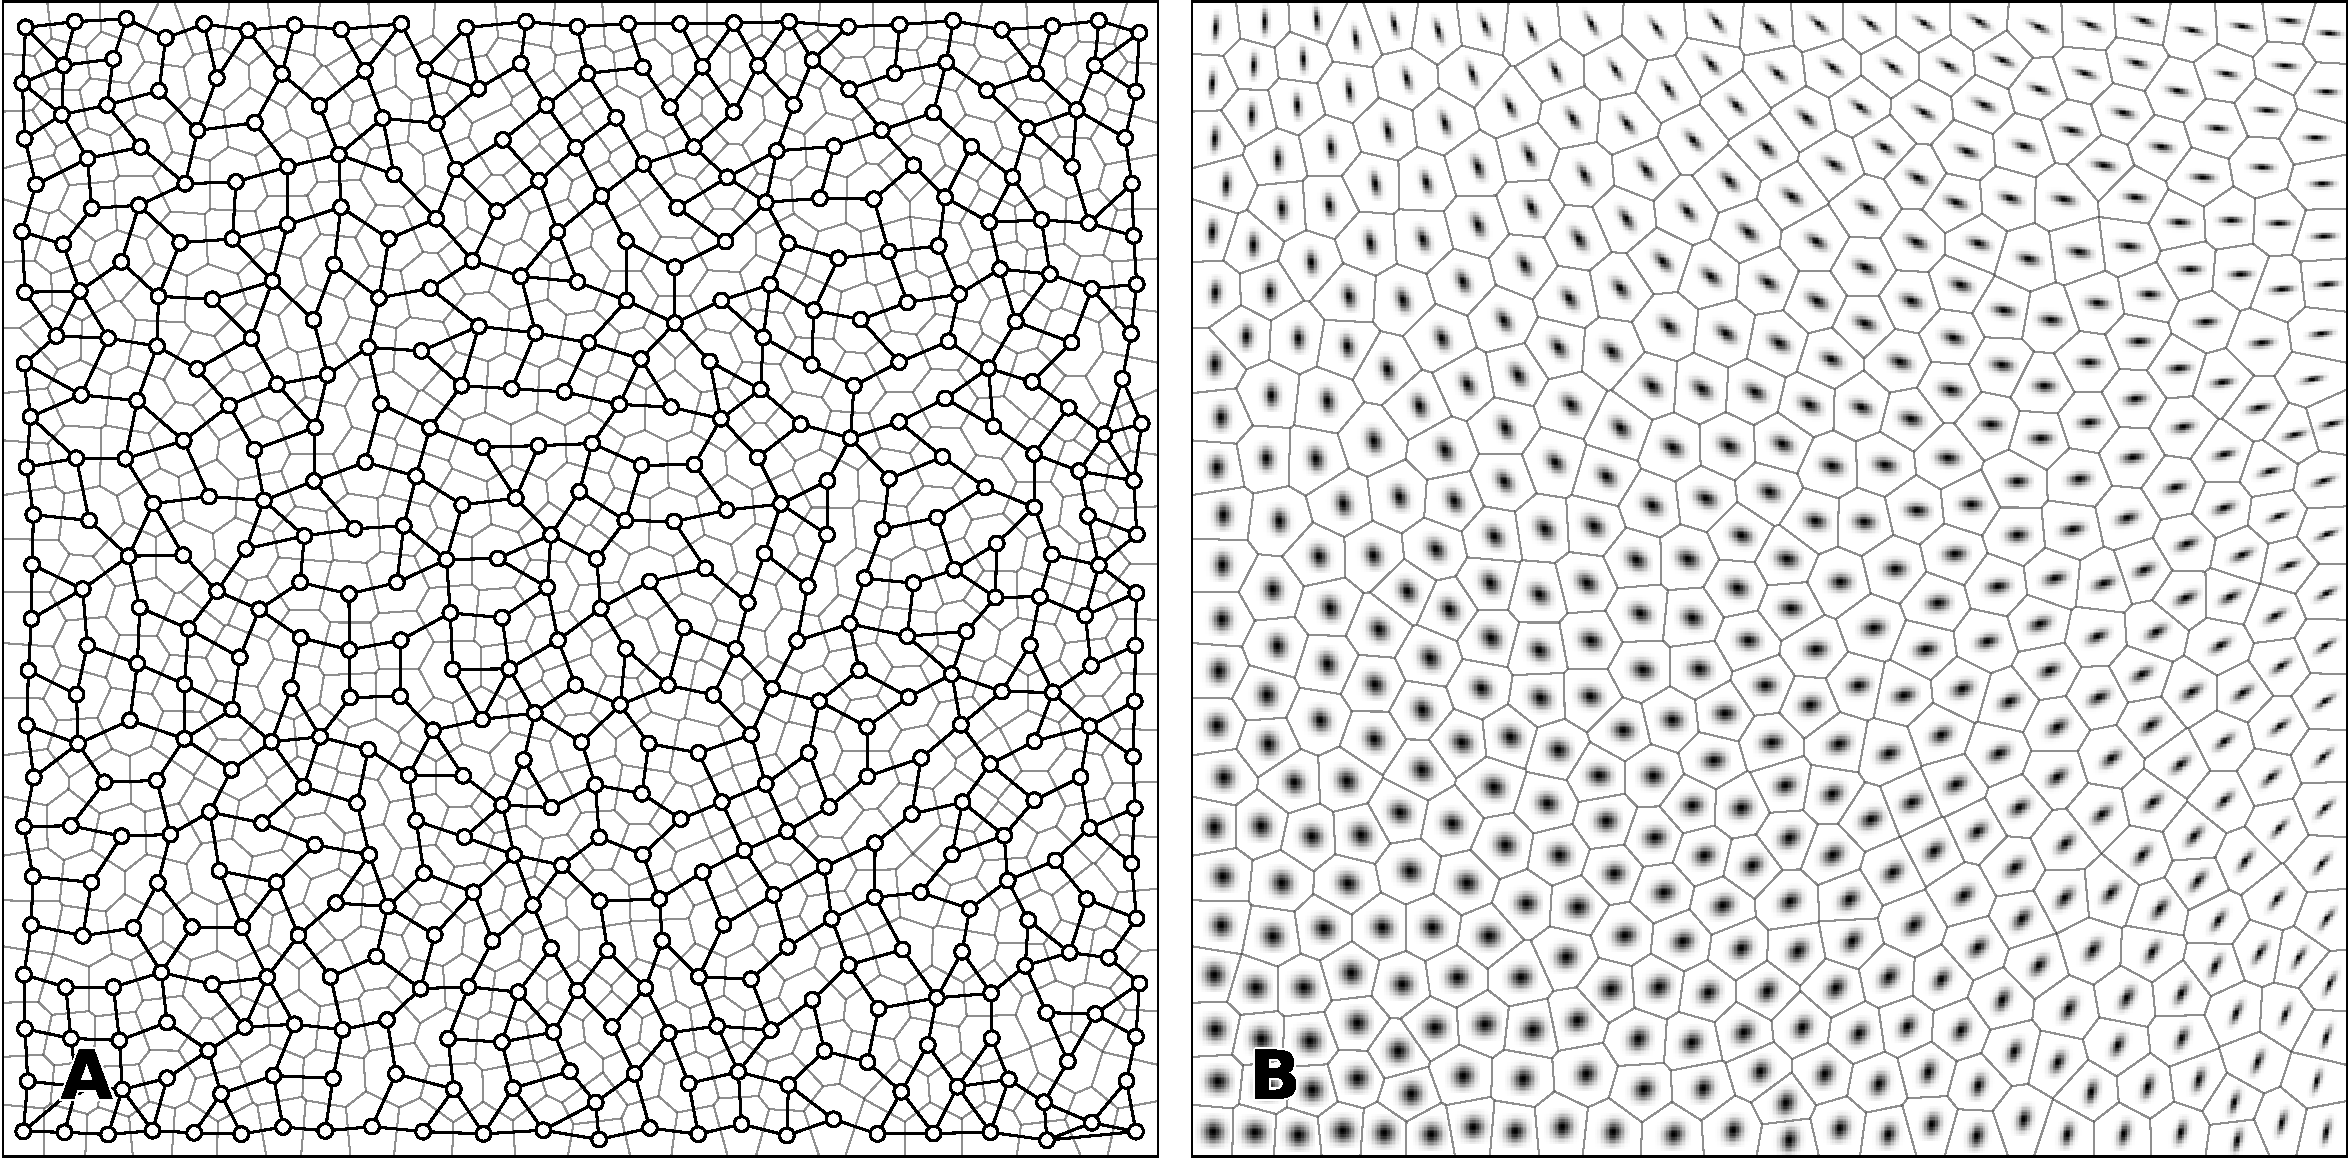
\includegraphics[width=\columnwidth]{figures/vsom-gaussian-1.pdf}
  
%%   \vspace{2mm}
  
%%   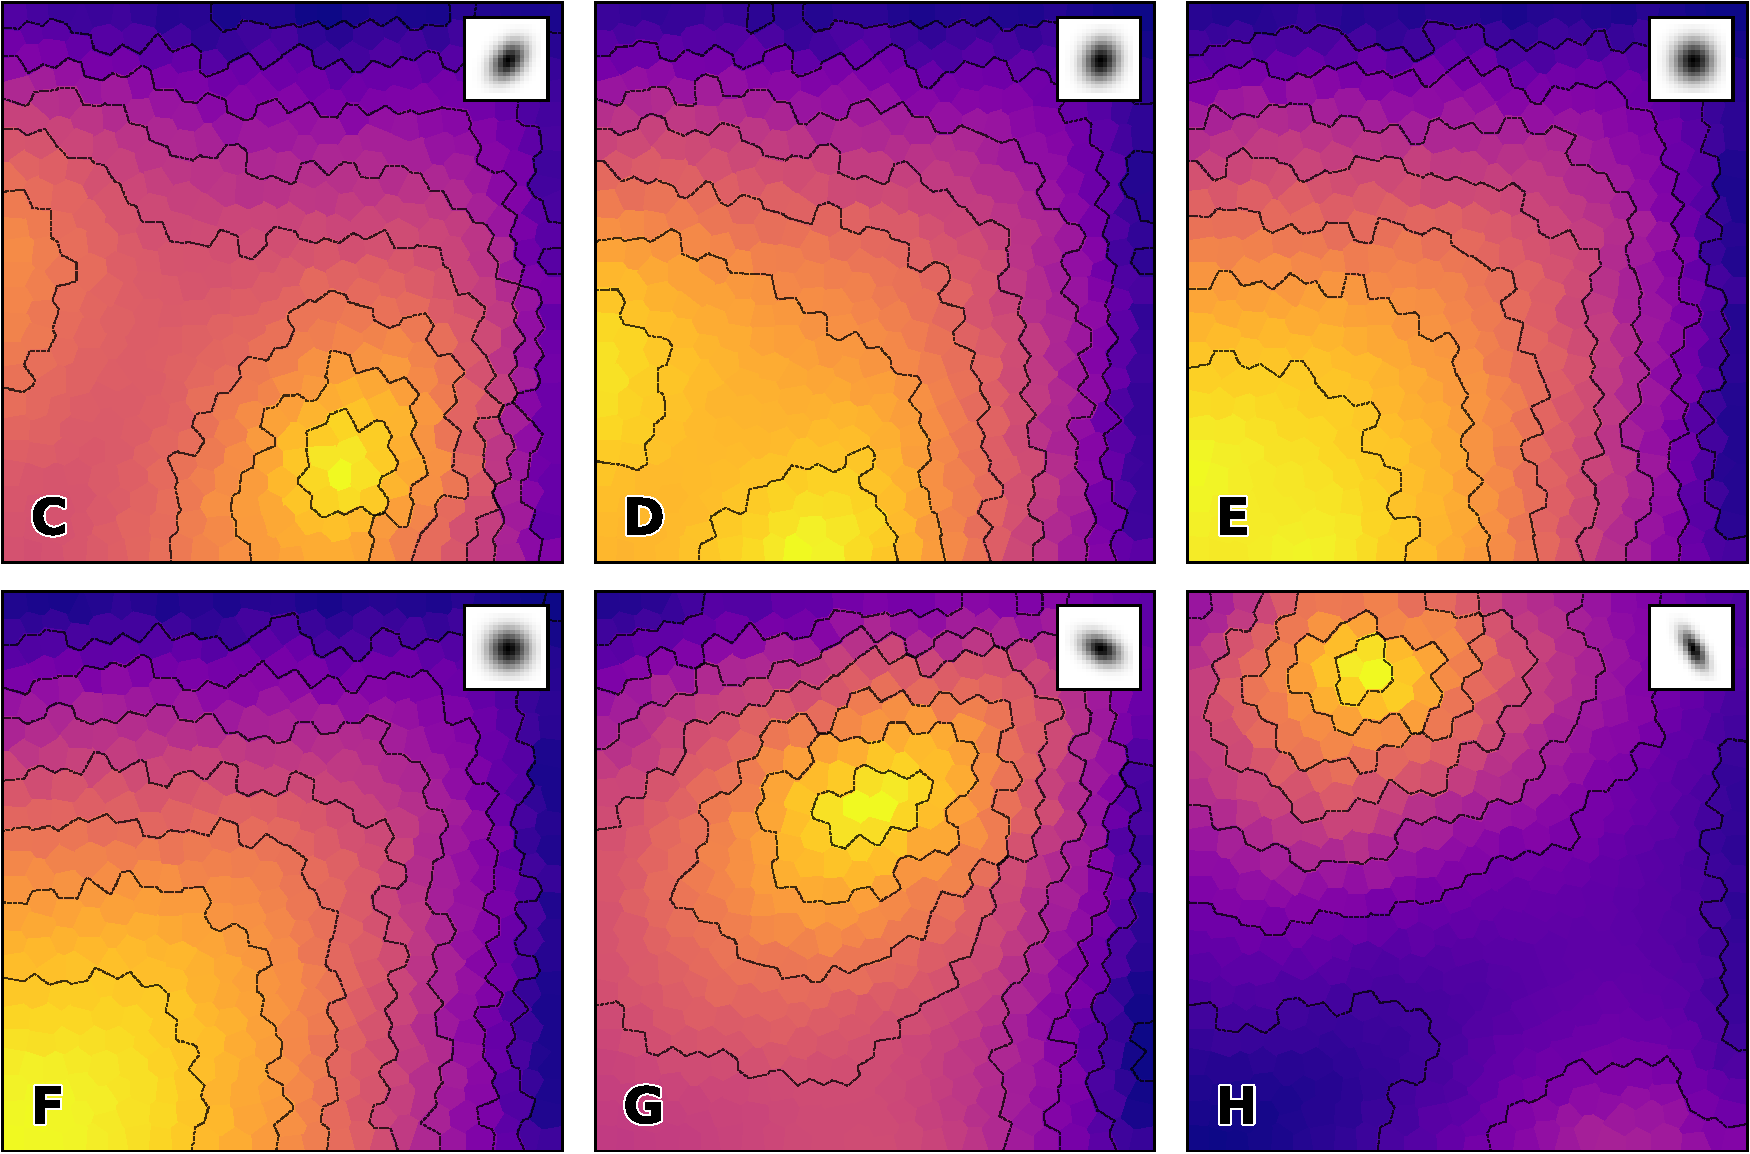
\includegraphics[width=\columnwidth]{figures/vsom-gaussian-2.pdf}

%%   \vspace{2mm}

%%   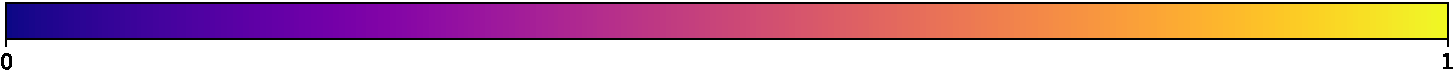
\includegraphics[width=\columnwidth]{figures/colormap.pdf}

%%   \caption{}
%% \end{figure}
